% Shared physical model and recovery protocol for the first roadmap stage.
\documentclass[11pt,a4paper]{ctexart}
\usepackage[margin=2cm]{geometry}
\usepackage{amsmath,amssymb,booktabs,tabularx,graphicx}
\usepackage[colorlinks=true,urlcolor=blue]{hyperref}
\setlength{\parindent}{2em}
\setlength{\parskip}{3pt}
\title{IMU--UWB 不变定位：第一阶段共同协议与恢复比较}
\author{Codex}
\date{2026年11月4日}
\begin{document}
\maketitle
\section{本轮推进及原论文对照}
Oursland 与 Mehrabian (2024) 研究 $SE_2(3)$ 上的 IMU--UWB TDoA 融合与大航向初差。
当前恢复研究延续 IMU--UWB 不变定位主题，但使用真实 TWR 距离，\textbf{不能与原文 TDoA 数字直接排名}。
本轮建立同状态、同物理先验、同输入、同离散噪声的 InEKF-15／ESKF-15，
并对完整 deep 与固定捕获初始化／中断后重置进行配对。
这是实验基线与实现一致性的完善，尚不构成新的收敛定理。

与旧代码先给物理对角先验、再用 Adjoint 转换量测的做法相比，
本轮显式定义物理误差到群误差的映射，直接验证完整量测与重置雅可比。
共同离散模型与历史 TWR 协方差实现有所不同，旧结果不覆盖，不将本轮变化只归因于监督器。

\section{共同名义传播与噪声}
设 $X=(R,v,p)$，IMU 已转为 SI 单位，$a=a_m-b_a$，$\omega=\omega_m-b_g$，
$g=(0,0,-9.81)^\top$。双方使用区间起点姿态冻结的同一个离散步：
\begin{align}
R^+&=R\operatorname{Exp}([\omega\Delta t]_\times),\\
v^+&=v+(Ra+g)\Delta t,\\
p^+&=p+v\Delta t+\tfrac12(Ra+g)\Delta t^2.
\end{align}
不加入高度截断或真值高度伪量测；该步不等于旋转区间内的高阶闭式积分。
物理误差为真值减估计：
\begin{equation}
e=[\delta\theta_b,\delta v_w,\delta p_w,\delta b_g,\delta b_a]^\top.
\end{equation}
姿态使用乘法误差 $R_{\rm true}=\hat R\operatorname{Exp}(\delta\theta_b)$。
令 $\phi=\omega\Delta t$、$E=\operatorname{Exp}([\phi]_\times)$，上述离散名义步的精确一阶雅可比为
\begin{equation}
F_e=\begin{bmatrix}
E^\top&0&0&-J_r(\phi)\Delta t&0\\
-R[a]_\times\Delta t&I&0&0&-R\Delta t\\
-\frac12R[a]_\times\Delta t^2&I\Delta t&I&0&-\frac12R\Delta t^2\\
0&0&0&I&0\\0&0&0&0&I
\end{bmatrix}.
\end{equation}
共享独立噪声顺序为陀螺、加计、陀螺偏置率、加计偏置率，映射
\begin{equation}
G_e=\begin{bmatrix}
-J_r(\phi)\Delta t&0&0&0\\
0&-R\Delta t&0&0\\
0&-\frac12R\Delta t^2&0&0\\
0&0&I\Delta t&0\\0&0&0&I\Delta t
\end{bmatrix},\qquad Q_e=G_eWG_e^\top.
\end{equation}
沿用历史参数的\textbf{逐采样率噪声}解释；偏置率在步末形成增量，方差随 $\Delta t^2$ 缩放。
这不是连续时间功率谱密度模型，也未通过真实偏置真值或 NEES 校准。

\section{不变误差、观测和重置}
本轮采用真值相对估计的右不变误差 $X_{\rm true}\hat X^{-1}$。
相应预测、观测和注入均使用同一约定。
物理误差到左注入群误差 $\xi$ 的一阶映射为
\begin{equation}
\xi=C(X)e,\quad C(X)=\begin{bmatrix}
R&0&0&0&0\\{}[v]_\times R&I&0&0&0\\{}[p]_\times R&0&I&0&0\\
0&0&0&I&0\\0&0&0&0&I
\end{bmatrix}.
\end{equation}
因此同一个物理先验和离散噪声在不变坐标下为
\begin{align}
P_{r0}&=C(X_0)P_{e0}C(X_0)^\top,\\
F_r&=C(X^+)F_eC(X)^{-1},\qquad Q_r=C(X^+)Q_eC(X^+)^\top.
\end{align}
实现先在物理坐标传播，再映射回不变坐标；与上述公式等价。
这保证比较没有暗中改变 IMU 噪声，不宣称完整有偏系统的误差动力学自治。

本数据协议使用零杆臂 TWR：
\begin{align}
z_i=\|p-a_i\|+\beta_i+n_i,\quad
q_i^\top&=\frac{(p-a_i)^\top}{\|p-a_i\|},\\
H_e&=[0\ \ 0\ \ q_i^\top\ \ 0\ \ 0],\\
H_r&=[-q_i^\top[p]_\times\ \ 0\ \ q_i^\top\ \ 0\ \ 0].
\end{align}
两个 15 维原始距离 tracker 以 $\nu=z_i-\beta_i-\hat r_i$ 和
$S=HPH^\top+\sigma_i^2$ 计算 NIS。
前 256 次有效更新预热；其后 NIS 大于 $3.5^2$ 拒绝，接受样本用
$w=\min(1,2/\sqrt{\mathrm{NIS}})$、$R_{\rm eff}=\sigma_i^2/w$ 降权。
所有方法与 deep 两支路共享原始测距偏置、标准差和鲁棒规则；提升支路按半平方观测传播量测方差。

ESKF 右乘姿态／加性平移注入，不变滤波器左乘 $SE_2(3)$ 注入：
\begin{equation}
R_{e}^+=R_e\operatorname{Exp}(\delta\theta_b),\qquad
X_r^+=\operatorname{Exp}_{SE_2(3)}(\delta\xi)X_r.
\end{equation}
Joseph 后验协方差分别通过
$\operatorname{diag}(J_r(\delta\theta_b),I_{12})$ 和
$\operatorname{diag}(J_l^{SE_2(3)}(\delta\xi),I_6)$ 重置。
传播、测距和重置均经过中心差分；共同预测协方差与世界坐标平移检查通过。
大旋转修正时用增广矩阵指数计算群左雅可比，避免固定阶幂级数截断失真：
\begin{equation}
J_l(A)=\int_0^1\exp(sA)\,ds
=\left[\exp\begin{pmatrix}A&I\\0&0\end{pmatrix}\right]_{1:9,10:18},
\qquad A=\operatorname{ad}_{\delta\xi}.
\end{equation}
此处修复的是数值计算。即使同一个物理增益给出 $\delta p_w$，有限群注入仍满足
$p^+=p+J_l^{SO(3)}(\delta\xi_\theta)\delta p_w$，与 ESKF 的直接加性修正不同。
大姿态修正可旋转或削弱平移修正；准确重置并不保证大误差高斯线性化有效。

\section{捕获与简化基线}
提升观测沿用 $[q,s,h,p,v,1]$，$q=\frac12p^\top p$、$s=p^\top v$、$h=v^\top v$：
\begin{equation}
y_i=\tfrac12((z_i-\beta_i)^2-\sigma_i^2)-\tfrac12 a_i^\top a_i
=q-a_i^\top p+\epsilon_i.
\end{equation}
提升 capture 使用半平方创新与量测值代入的方差
$V_i=(z_i-\beta_i)^2\sigma_i^2+\tfrac12\sigma_i^4$，再形成自己的 NIS。
因此提升与原始测距的数值创新及方差单位不同，不能直接混为同一统计量。
完整 deep 保留独立捕获和原始距离 tracker；简化方案只捕获 2 秒，然后停止捕获、保留一个 tracker。
reset 方案在测距恢复供数时额外重新捕获 2 秒。
各捕获方案共享提升块 $p/v/q/s/h$ 标准差 $8/2/80/40/20$，
世界加速度不确定度为 $10$ m/s$^2$；该提升块不是与 15 维 IMU 核相同的过程协方差。
完整 deep 沿用历史监督参数（含最少 20 秒捕获输出驻留），本轮没有按测试结果调优。
交接先在\textbf{物理坐标}组合捕获的平移块与 IMU 核的姿态／偏置块，再以新状态的 $C(X)$ 映射；
不能直接把世界平移方差塞入不变坐标。
此保守分块仍缺共享量测的互相关，deep 混合输出也没有严格融合协方差。

\section{冻结协议与判定}
12 条真实 TWR 日志均采于 2021-02-12，含六种运动、每种两条。
每类第一条训练、第二条评估，训练拟合逐锚中位偏置和 $1.4826\operatorname{MAD}$，
标准差限制在 $[0.08,0.50]$ m；另提供 12 条 LOSO 对照。
IMU/TWR 共同相对 OptiTrack 校正历史冻结的 0.20 s，不逐日志调时延。
前 1.5 秒 IMU 用于初始重力对准与偏置估计，计分从随后样本开始。
受控初始位置为首个计分位置真值加偏移，因此\textbf{不是无真值冷启动}。
90/180 度为相对于共同初始重力对准姿态的 yaw 扰动；本数据无真实姿态，不能把它称为已知绝对航向误差。

\begin{center}
\begin{tabular}{lrr}
\toprule
用例组&条件数&五种方法评估数\\\midrule
12 条 LOSO，0／9 m&24&120\\
6 条固定留出，0--12 m、三方向、yaw 扰动&90&450\\
6 条测距中断，15--25 秒、0／9 m&12&60\\\midrule
合计&126&630\\\bottomrule
\end{tabular}
\end{center}
首次 1 秒阈内驻留只作辅助指标。
令 $e_p(t)=\|\hat p-p_{\rm GT}\|$，$t_0=0$ 或测距恢复供数时刻，稳定恢复为
\begin{equation}
t_s=\inf\{t\ge t_0:\ \forall \tau\in[t,T],\ e_p(\tau)\le0.5\text{ m},\ T-t\ge5\text{ s}\}.
\end{equation}
不存在符合条件的后缀则失败，保留完整有限误差和末段 RMSE；
中断恢复计时为 $t_s-t_0$，不把中断本身的 10 秒混入恢复延迟。
此定义是离线后验，不是在线监督器使用真值。
统计按完整日志配对并重采样日志；不能将相关的 IMU 样本当独立试验。
日志同日、且旧监督器开发看过全部 12 条，留出只隔离本轮标定，\textbf{不能主张独立日期泛化}。

\section{实测结果与第一阶段决策}
% Verified numerical results and the conditional first-stage decision.
630 行方法结果、126 条完整历史均通过独立重算，全部位置／速度输出有限；
CSV 与重算的最大绝对差为 $3.64\times10^{-12}$。
\textbf{有限数值不等于可靠定位}：InEKF 与 ESKF 的最坏位置误差分别约 22.0 km、8.07 km，
均保留为失败，不裁去后半轨迹。

\begin{center}
\begin{tabular}{lrrr}
\toprule
方法&LOSO 成功／24&留出成功／90&中断成功／12\\\midrule
InEKF-15&17&62&5\\
ESKF-15&20&76&3\\
捕获初始化&20&75&8\\
捕获初始化＋中断重置&20&75&10\\
完整 deep&19&61&2\\\bottomrule
\end{tabular}
\end{center}

留出组完整位置 RMSE 中位数：捕获初始化 0.331 m、deep 0.375 m；
末 5 秒分别 0.151 m、0.179 m。
按日志等权的配对完整 RMSE 相对变化为 deep 高 10.76\%，
日志重采样 95\% 区间为 $[1.64,17.02]\%$。
成功率差为 $-15.56$ 个百分点，但六日志重采样区间 $[-61.11,28.89]$ 跨零；
不将相关的 90 个用例当独立证据。
双方均成功的 48 对中，日志等权恢复时间差为 deep 慢 3.75 s，
可用五日志的区间为 $[0.006,11.20]$ s；条件化统计不能代表全部失败用例。

deep \textbf{存在局部收益}：留出 square 日志成功 13/15，而捕获初始化为 0/15；
同时 octagon／star 分别由简化方案的 15/15 降为 deep 的 2/15、1/15。
与简化初始化配对，deep 独有成功 13 对、简化独有成功 27 对。
90／180 度扰动下 ESKF 均 6/6，简化初始化均 5/6，deep 为 4/6、5/6；
普通 InEKF 为 4/6、3/6。这是当前零杆臂 TWR 共同模型结果，不能推广为对原文 TDoA 的否定。

中断后 deep／简化重置的末 5 秒位置 RMSE 中位数为 9.235／0.151 m。
deep 两次成功均来自 square，恰为重置失败的两例；重置其余十例成功，deep 全部失败。
双方没有共同成功对，因此\textbf{不存在可计算的配对成功恢复时间差}。
分别报告的成功用例中位恢复时间为 11.79／11.10 s，不能据此称速度相当。

\textbf{第一阶段工程与比较工作完成，第二阶段的进入条件未满足。}
保留完整 deep 及其局部收益证据，但暂停以当前双滤波器为核心的稳定优势叙事。
目前优先基线是固定捕获初始化、测距恢复后再次捕获与单不变 tracker。
它仍有 square 失败和正常初期峰值，尚未达到普遍可靠定位。
若继续研究，应先解释“square 改善、octagon／star 退化、长中断捕获漂移”这一具体机制，
再以独立日期与锚点几何检验；本轮没有新增收敛定理、NEES 或目标硬件实时证据。

\clearpage
\section{可观察结果}
\begin{center}
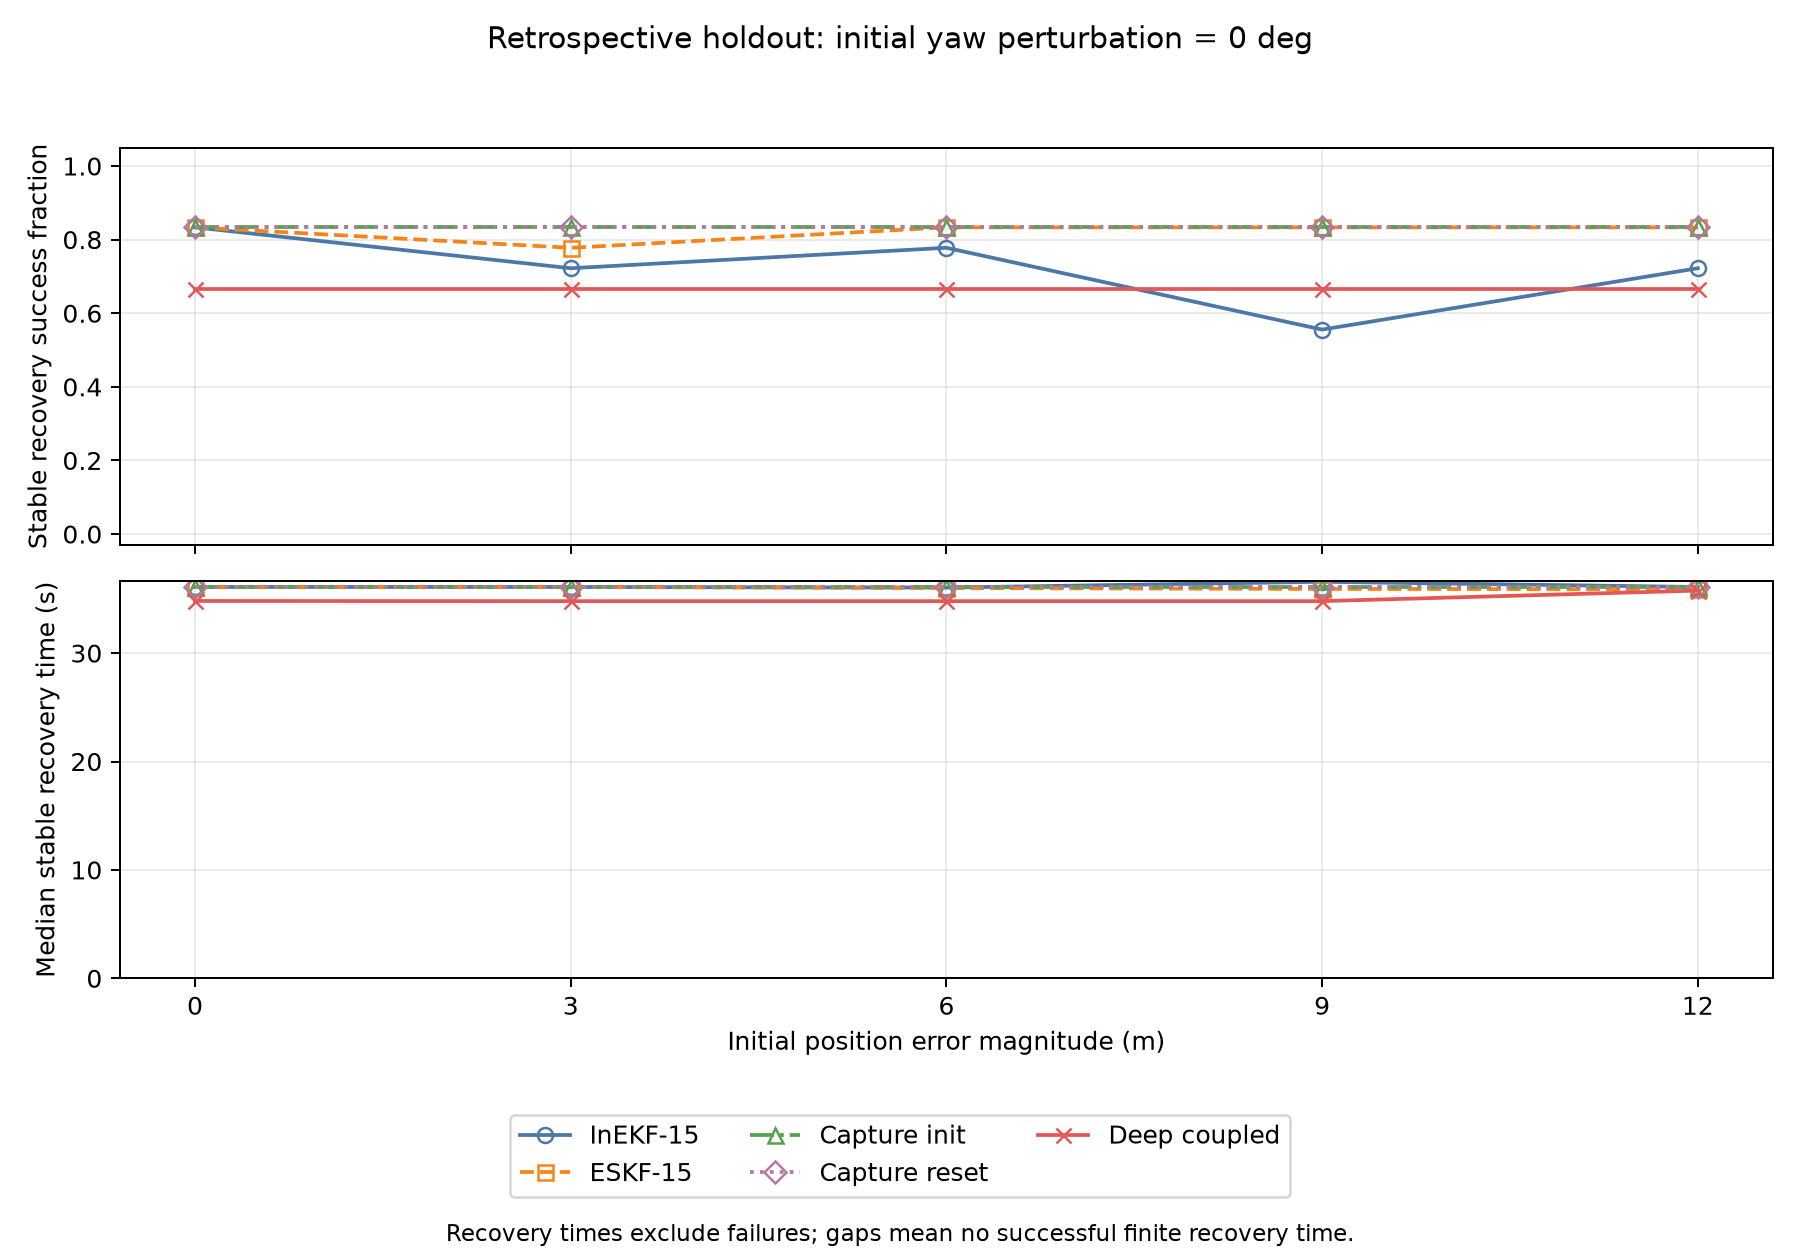
\includegraphics[width=0.87\linewidth]{../imu-uwb-inekf/results/roadmap_stage1_20261104_final/holdout_capture_domain.png}
\end{center}
固定标定留出组的初差域。0 m 为六条件，非零幅度均为六日志乘三方向。
下图仅对成功用例统计，约 35--36 秒的终段稳定时间不等于首次达到阈值。

\begin{center}
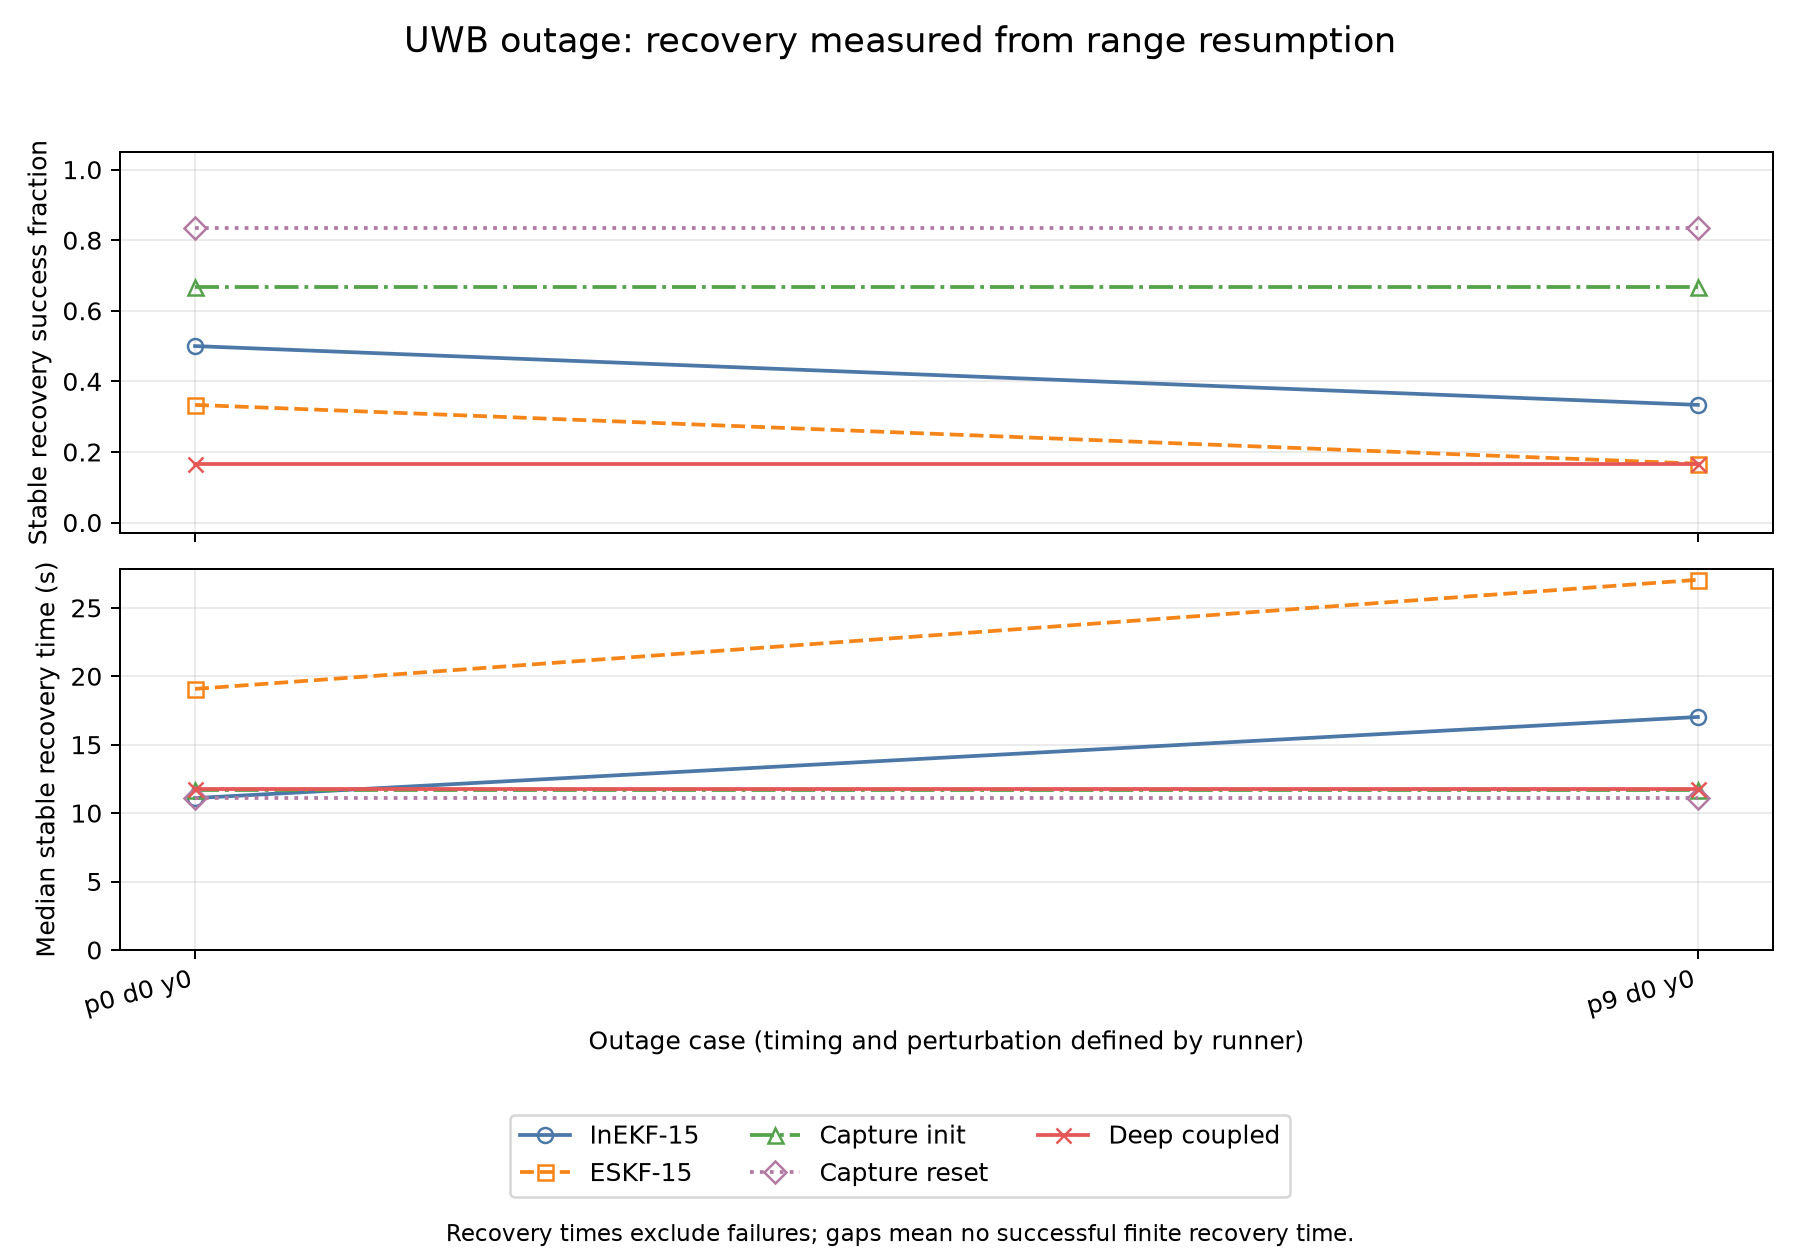
\includegraphics[width=0.87\linewidth]{../imu-uwb-inekf/results/roadmap_stage1_20261104_final/outage_recovery.png}
\end{center}
测距中断 15--25 秒；恢复时间从 25 秒起算，每组六条件。
失败不会获赋一个虚构恢复时间。

\clearpage
\section{失败与局部收益并列检查}
\begin{center}
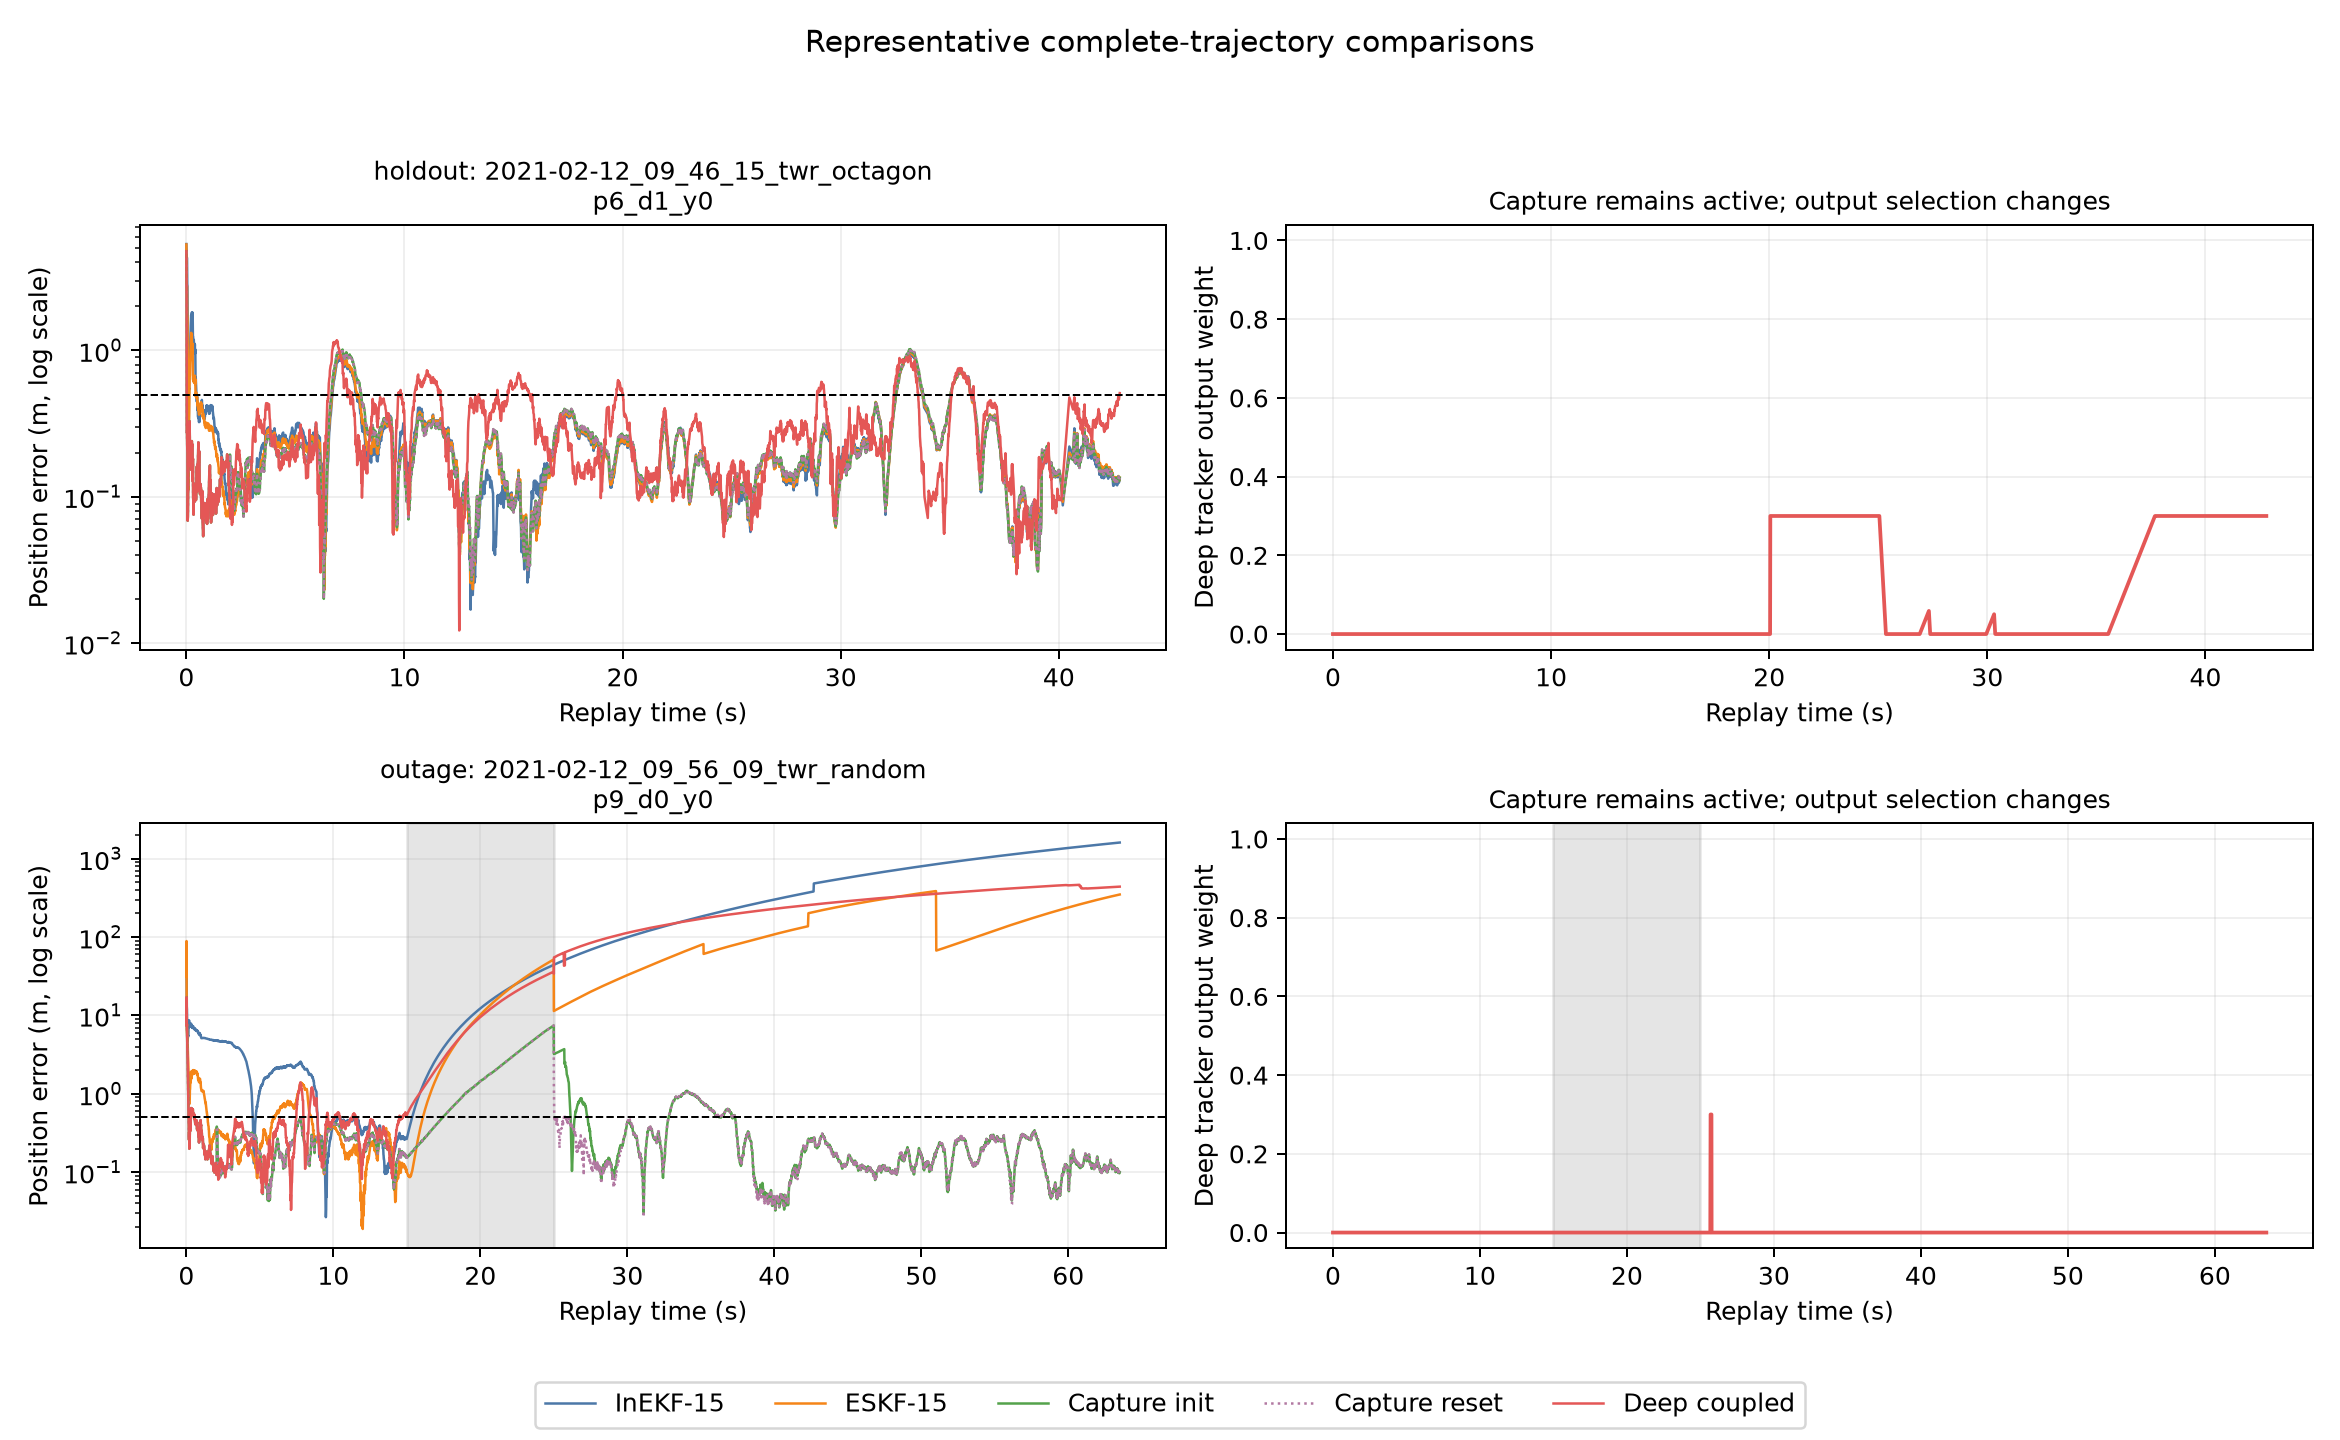
\includegraphics[width=\linewidth]{../imu-uwb-inekf/results/roadmap_stage1_20261104_final/representative_failures.png}
\end{center}
保留完整误差及 deep 输出权重。octagon 的输出混合产生额外末段代价；
random 中断后 deep 权重大多为零，持续捕获仍可漂移。
后者是观察到的现象，不能仅凭曲线证明全部内部因果。

\begin{center}
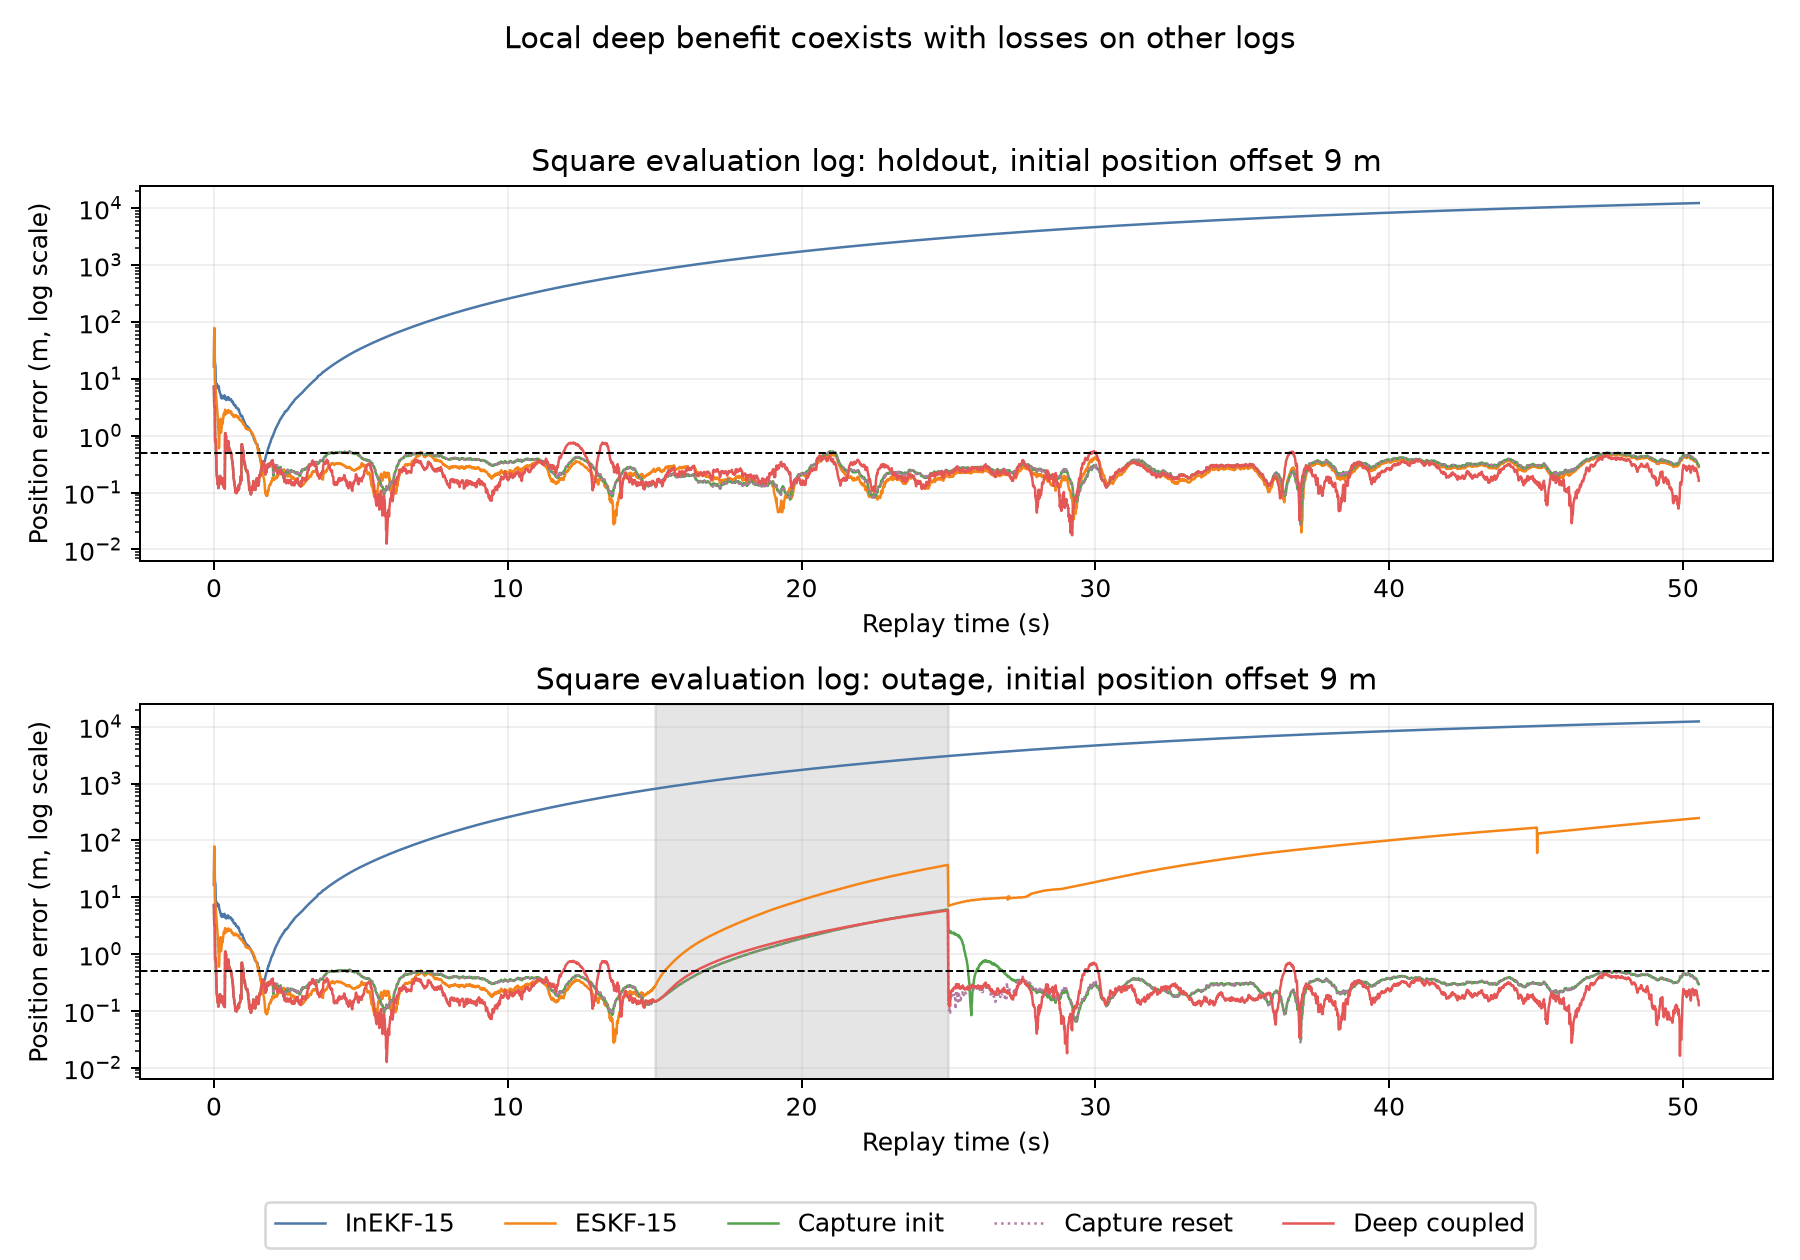
\includegraphics[width=0.83\linewidth]{../imu-uwb-inekf/results/roadmap_stage1_20261104_final/deep_local_gain.png}
\end{center}
square 的 deep 局部收益明确保留；少数阈值峰值可导致简化方案稳定后缀判定失败，
必须结合末段误差、完整峰值和成功率解释。


\end{document}
